% --- Figure: bridge-supremum-to-convergence.tex ---
% Requires: \usepackage{tikz}, \usepackage{amsmath}

\begin{figure}[H]
  \centering
  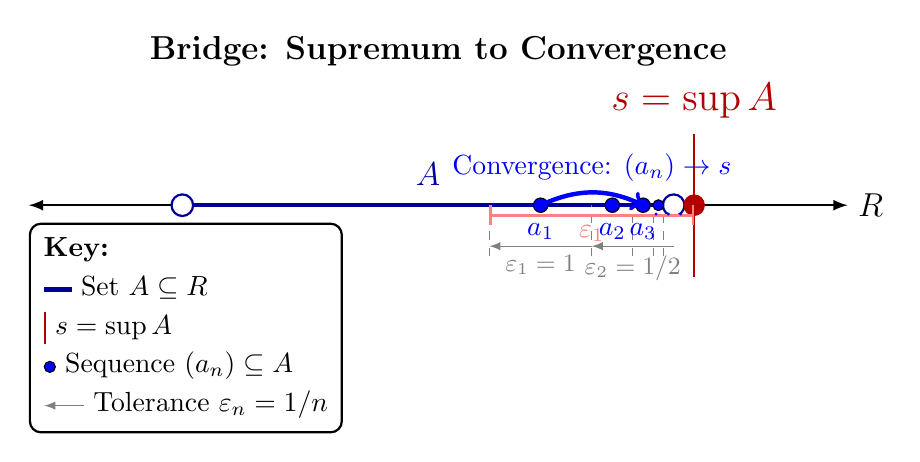
\begin{tikzpicture}[scale=1.3]

    % Main Axis
    \draw[latex-latex, thick] (-1.5,0) -- (6.5,0) node[right, font=\large] {$\mathbb{R}$};

    % The Set A (a generic interval [a, s))
    \draw[ultra thick, blue!60!black, line cap=rect] (0,0) -- (4.8,0);
    \node[blue!60!black, above] at (2.4,0.1) {\large $A$};
    \fill[white, draw=blue!60!black, thick] (0,0) circle (3pt); % Open boundary at left (optional)
    \fill[white, draw=blue!60!black, thick] (4.8,0) circle (3pt); % Open boundary at right (crucial)

    % The Supremum s
    \draw[thick, red!70!black] (5, -0.7) -- (5, 0.7);
    \fill[red!70!black] (5,0) circle (3pt);
    \node[red!70!black, above, yshift=2pt] at (5,0.7) {\Large $s = \sup A$};

    % The decreasing tolerance markers (epsilon_n = 1/n)
    \foreach \n/\val in {1/3.0, 2/4.0, 3/4.4, 4/4.6, 5/4.7} {
        \draw[dashed, thin, gray] (\val, -0.5) -- (\val, 0);
    }
    \draw[latex-, thin, gray] (3.0, -0.4) -- (4.0, -0.4) node[midway, below, gray, font=\small] {$\varepsilon_1 = 1$};
    \draw[latex-, thin, gray] (4.0, -0.4) -- (4.8, -0.4) node[midway, below, gray, font=\small] {$\varepsilon_2 = 1/2$};

    % Step 1: Tolerance is s - epsilon_1
    \coordinate (T1) at (3,0);
    \draw[thick, red!50, |-|] (3,-0.1) -- (5,-0.1);
    \node[red!50, below] at (4,-0.1) {$\varepsilon_1$};

    % Constructing the sequence (a_n) in A
    % a_1 found in A beyond s - epsilon_1
    \coordinate (a1) at (3.5,0);
    \fill[blue, draw=black] (a1) circle (2pt);
    \node[blue, below, yshift=-3pt] at (a1) {$a_1$};

    % a_2 found in A beyond s - epsilon_2
    \coordinate (a2) at (4.2,0);
    \fill[blue, draw=black] (a2) circle (2pt);
    \node[blue, below, yshift=-3pt] at (a2) {$a_2$};

    % a_3 found in A beyond s - epsilon_3
    \coordinate (a3) at (4.5,0);
    \fill[blue, draw=black] (a3) circle (2pt);
    \node[blue, below, yshift=-3pt] at (a3) {$a_3$};

    % a_4 found in A beyond s - epsilon_4
    \coordinate (a4) at (4.65,0);
    \fill[blue, draw=black] (a4) circle (1.5pt);

    % Dots indicating sequence continuing
    \node[blue] at (4.75, -0.1) {$\cdots$};

    % The convergence arrow
    \draw[->, ultra thick, blue, bend left=25] (a1) to node[midway, above, blue] {Convergence: $(a_n) \to s$} (a3);


    % Title
    \node[align=center, font=\large] at (2.5, 1.5) {\textbf{Bridge: Supremum to Convergence}};
% Legend/Key
\node[draw, thick, rounded corners, inner sep=5pt, right, align=left] at (-1.5, -1.2) {
    \textbf{Key:}\\[2pt]
    \tikz[baseline=-0.5ex]{\draw[ultra thick, blue!60!black, line cap=rect] (0,0) -- (0.3,0);} Set $A \subseteq \mathbb{R}$\\[2pt]
    \tikz[baseline=-0.5ex]{\draw[thick, red!70!black] (0, -0.2) -- (0, 0.2);} $s = \sup A$\\[2pt]
    \tikz[baseline=-0.5ex]{\fill[blue, draw=black] (0,0) circle (2pt);} Sequence $(a_n) \subseteq A$\\[2pt]
    \tikz[baseline=-0.5ex]{\draw[latex-, thin, gray] (0, 0) -- (0.5, 0);} Tolerance $\varepsilon_n = 1/n$
};
  \end{tikzpicture}
  \caption{Illustrating the constructive connection between the static existence of a supremum ($s$) and the dynamic process of convergence. The $\varepsilon$-characterization acts as a sequence generator. By selecting decreasing tolerances $\varepsilon_n = 1/n$, we are guaranteed to find corresponding elements $a_n \in A$ that satisfy $s - \frac{1}{n} < a_n \le s$. The sequence $(a_n)$, contained strictly within $A$, is forced by the 'squeeze' of the tolerances to converge to $s$ as $n \to \infty$. This construction provides the required sequence $(a_n) \subseteq A$ such that $\lim_{n \to \infty} a_n = \sup A$.}
  \label{fig:bridge-supremum-to-convergence}
\end{figure}